%!TEX root = tukedip.tex
\section{Anal\'yza}

Text záverečnej práce obsahuje kapitolu, v~rámci ktorej autor uvedie
analýzu riešených problémov. Táto kapitola môže byť v~prípade potreby
delená do viacerých podkapitol. Autor v~texte záverečnej práce môže
zvýrazniť kľúčové slová, pričom sa použije príslušný štýl pre kľúčové
slová -- napr. toto je kľúčové slovo. V~texte môžu byť použité obrázky
a~tabuľky podľa nasledujúcich príkladov:

\begin{figure}[!ht]
\centering \unitlength=1mm
\begin{picture}(30,30)(0,0)
\put(0,0){\line(1,0){30}}
\put(0,0){\line(0,1){30}}
\put(30,0){\line(0,1){30}}
\put(0,30){\line(1,0){30}}
\end{picture}
\caption{Toto je štvorec}\label{o:1}
\end{figure}


Obrázok by mal byť podľa možnosti centrovaný. Pri jeho opisovaní
v~texte treba použiť odkazy na obrázok v~tvare Obrázok~\ref{o:1}.

\tabcolsep=8pt
\begin{table}[!ht]\caption{Prehľad jednotiek}\label{t:1}
\smallskip
\centering
\begin{tabular}{|l|c|} \hline
Názov	& (Jednotka v~sústave SI) \\ \hline
Napätie & $\upmu$V \\ \hline
\end{tabular}
\end{table}
\nomenclature{$\upmu$}{mikro, $10^{-6}$}
\nomenclature{SI}{Syst\`eme International}
\nomenclature{V}{volt, základná jednotka napätia v sústave SI}

Tabuľka by mala byť podľa možnosti centrovaná. Pri jej opisovaní
v~texte treba použiť odkazy na tabuľku v~tvare: pozri
Tabuľku~\ref{t:1}. Na číslovanie obrázkov, resp. tabuliek treba použiť
triedenie. Za slovom {\it Obrázok} nasleduje ako prvé číslo kapitoly
alebo časti, v~ktorej sa obrázok nachádza, potom medzera, pomlčka,
medzera a~poradové číslo ilustrácie v~danej kapitole alebo časti.
Napr.:~Obrázok~\ref{o:1} (čiže: prvý obrázok v~druhej kapitole alebo
časti). V~prípade, ak tabuľka presahuje stranu, je možné použiť balík
\verb+longtable+.

Navrhujeme zaraďovať obrázky v~elektronickej podobe. Napríklad
Obrázok~\ref{o:2}, ktorý opisuje riešenie diferenciálnej rovnice
tlmených oscilácií
%% \def\ud{\mathrm{d}}
\begin{equation}\label{r:1}
\frac{\ud^2y}{\ud t^2}+\frac{\ud y}{\ud t}+y =0, \qquad y(0)=1, \quad
y\,'(0)=15,
\end{equation}
bol vytvorený v~MATLABe a~príkazom \texttt{print tlmosc.eps -f1
-deps2} bol uložený vo formáte Encapsulated Postscript. Na prípadné
použitie pdf\LaTeX{}u sa obrázok konvertuje do formátu PDF, napr.
pomocou programu \texttt{epstopdf}. Zvyčajne sa číslujú vzťahy, na
ktoré sa v~texte odvolávame. Napríklad: vzťahy (\ref{r:1}) definujú
Cauchyho začiatočnú úlohu.


\begin{figure}[ht!]
\centering
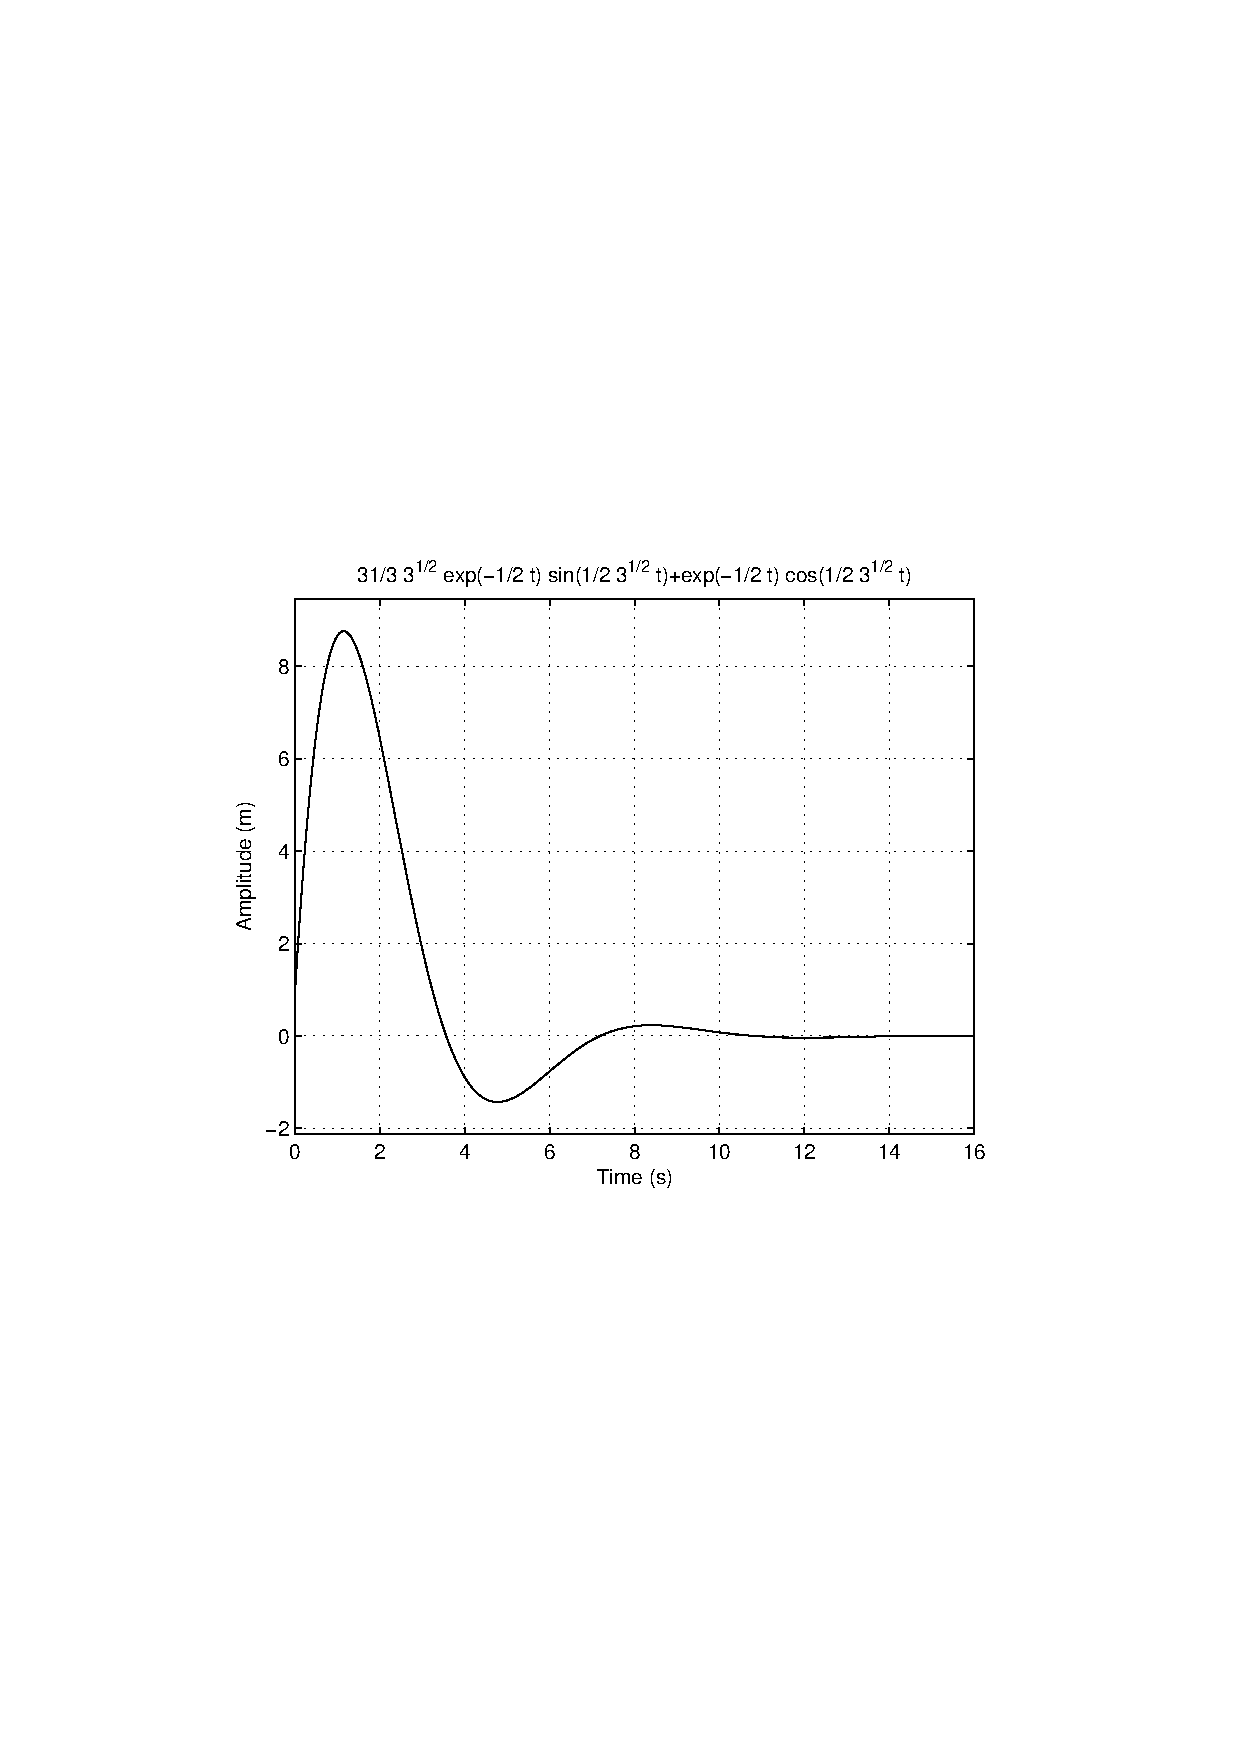
\includegraphics[width=0.7\textwidth]{tlmosc}
\caption{Grafické zobrazenie riešenia rovnice \ref{r:1}}\label{o:2}
\end{figure}



\subsection{Podkapitola}
Podkapitoly záverečnej práce majú za úlohu členenie textu záverečnej
práce s~cieľom, čo najväčšej prehľadnosti. Kapitol môže byť viacero
a~v~ich názvoch sa používa desatinné číslovanie.